
\section{Introduction}

As outlined in \ref{sec:electricity_price_forecasting} different types of models have been investigated for forecasting spot electricity prices. In this work forecasting models should be used that exhibit the following characteristics: 

\begin{itemize}
	\item computationally lightweight
	\item capable of modeling seasonality
	\item capable of recognizing trends in the dataset
	\item good out-of-sample accuracy based on day ahead and real time electricity prices
	\item capable of being part of an automated model generation process
	\item accurate modeling of different energy price characteristics
\end{itemize}

Statistical models have been proven to provide good results and at the same time keeping the computational effort low \cite{aggarwal2009electricity,bunn2003forecasting}. In contrast structural or non-parametric models require additional input data and perform more complex operations such that they might not be the optimal choice for dynamic forecast environments. Therefore models in this work have been chosen from the well known set of parsimonious stochastic models. 

Different stochastic models are able to generate forecasts while considering existing seasonality in the data \cite{gould2008forecasting,de2011forecasting}. Examples of models exhibiting these characteristics are SARIMA, HoltWinters and TBATS, all of which are investigated in this work to evaluate their capability of forecasting on different settings and datasets. The best model is then chosen to provide forecasts for all simulations described later in this work. 

In general time series may be decomposed into seasonal, trend and cycle components which can be made use of by forecast models \cite{de2011forecasting}. Some models such as ARIMA and TBATS can handle existing trends in the dataset by applying transformations in a preprocessing step or by decomposing and separately modeling time series components. More simplistic models such as Simple Exponential Smoothing (SES) or pure Autoregressive (AR) models require the dataset to be stationary, i.e.~to exhibit a constant mean and variance \cite{weron2007modeling,hyndman2012forecasting}. In this case the dataset would have to be transformed before applying those models. 

Models should provide good out-of-sample accuracy which means that they need to be trained and tested on different datasets \cite{hyndman2012forecasting}. For example, considering training data from a training period of four weeks of energy price data and test data from a subsequent test period of one week a model is trained based on that training data but tested on the provided test data. Thus real life forecasting scenarios can be established and models are evaluated based on the accuracy on test datasets. A large scale evaluation of forecasting models based on different training and test datasets is presented later in this section. 

Building an automated model generation process is important for automatic model evaluation and model selection for simulations running over a longer period of time. As extensive simulations including forecasts represent a core contribution of this work an automated model generation process has been defined including preprocessing steps and model evaluation to find the best suited model for a given dataset. 

Inclusion of energy price characteristics such as mean reversion and price spikes into forecast model generation has been studied extensively considering different types of forecast models \cite{weron2008forecasting,bunn2003forecasting,aggarwal2009electricity}. Mean reversion denotes the characteristic that a time series returns to its mean after significant deviation. This characteristic is modeled by a AR(1) process and can be incorporated e.g.~into an ARIMA model. For handling price spikes three approaches have been defined in literature \cite{weron2008forecasting}: 1) Using models that allow spikes in input datasets 2) Remove price spikes completely from the data 3) Recognize and dampen observed spikes to mitigate their impact on out-of-sample forecasts. For simplicity reasons price spikes have not been modeled explicitly in this work meaning they are not dampened or removed from the datasets. 



\section{Methodology}

In this section the various methodologies used in the forecasting framework are discussed. 

%It presents seasonality estimation, time series decomposition, selected forecast models, model selection algorithm, the forecast simulation framework and a forecast model evaluation implemented on a large scale. 


\subsection{Seasonality estimation and periodogram}

Estimating seasonality is an important pre-processing step when building forecasting models. As most models are not able to automatically detect seasonality in the given data it is vital to determine possible seasonality cycles beforehand. 

One way of detecting seasonality in the data is by doing a spectral analysis for exploration of cyclical patterns. 
During the process the data is decomposed into underlying sinusoidal (sine and cosine) functions with particular wavelengths \cite{weron2007modeling}. 
The wavelength is commonly described as frequency which is the number of cycles per unit time. 

The frequency $\omega$ and the period $T$ have a reciprocal relationship $\omega = \frac{1}{T}$. Thus the period $T$ denotes the number of unit time stamps required to complete one period which in case of daily seasonality in a time series of hourly observations can be 24 time stamps, i.e.~24 hours. 

In order to visualize common frequencies a \textit{periodogram} may be generated which can be regarded as a tool for retrieving the most common frequencies from the dataset. As existing seasonality patterns in the data are likely to be detected by the periodogram as high valued frequencies it can be used to extract these frequencies and calculate the reciprocal as the seasonal period $T$. 

The formula of a periodogram for a vector of observations $\{x_1,\ldots,x_n\}$ is defined as \cite{weron2007modeling}:

		\[ I_n (w_k) = \frac{1}{n} \left| \sum_{t=1}^{n}{x_t  e^{-i(t-1) \omega_k} } \right|^2 \]
		
		where $\omega_k = 2 \pi (k/n)$ denote the Fourier frequencies in radians per unit time, $k = 1,\ldots,[n/2]$ and $[x]$ describes the largest integer value less than or equal to $x$. 

Figure \ref{fig:periodogram_July_2014} shows a periodogram of two weeks of hourly day ahead prices from the Nord Pool Spot power market. 
On the x-axis frequencies from 0 to 0.5 are displayed, on the y-axis each frequency's corresponding value is depicted, proportional to the number of occurrences of this frequency. In case of a random signal the frequencies should be uniformly distributed across the frequency scale. In this case clearly two frequency values stand out where the values are of magnitudes $\omega_1 = 0.0416$ and $\omega_2 = 0.0833$. This results in periods $T_1 = 24$ and $T_2 = 12$, which means that the underlying series exhibits a strong daily seasonality of 24 hourly prices with a so called \textit{harmonic} of 12 periods which denotes a multiple of the 24 hour period. 


\begin{figure}[htbp]
	\centering
		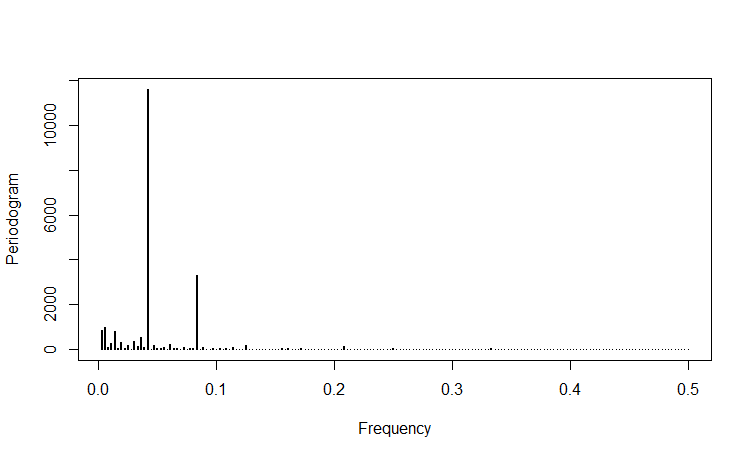
\includegraphics[width=0.8\textwidth]{figures/forecasting/periodogram_July_2014.png}
	\caption{Periodogram of hourly day ahead prices of Nord Pool Spot, Helsinki from July 7th to July 21st in 2014}
	\label{fig:periodogram_July_2014}
\end{figure}

After successfully determine meaningful seasonalities and their resulting periods from the dataset this information can be used to build forecast models that consider the respective seasonal periods in the model generation process. 



\subsection{Seasonal decomposition} \label{ssec:seasonal_decomposition}

Seasonal decomposition describes the process of decomposing a given time series into its components which are trend, seasonal or cyclic and irregular components. Decomposition is done by applying the STL model to the time series and extracting the above mentioned components where STL is defined as Seasonal-Trend decomposition procedure based on Loess \cite{cleveland1990stl}. 

The decomposition of a time series can be formalized as follows \cite{cleveland1990stl}: 

	\[ Y_v = T_v + S_v + R_v \]
	
where $Y_v$ denotes the original time series, $T_v$ the trend component, $S_v$ the seasonal component and $R_v$ the remainder component. $v \in \{ 1,\ldots,N \}$ denotes an individual time stamp in the series where $N$ is the number of unit time stamps in the time series. 

A sample seasonal decomposition of hourly time series is depicted in Figure \ref{fig:stl_decomposition_July_2014}. 

\begin{figure}[htbp]
	\centering
		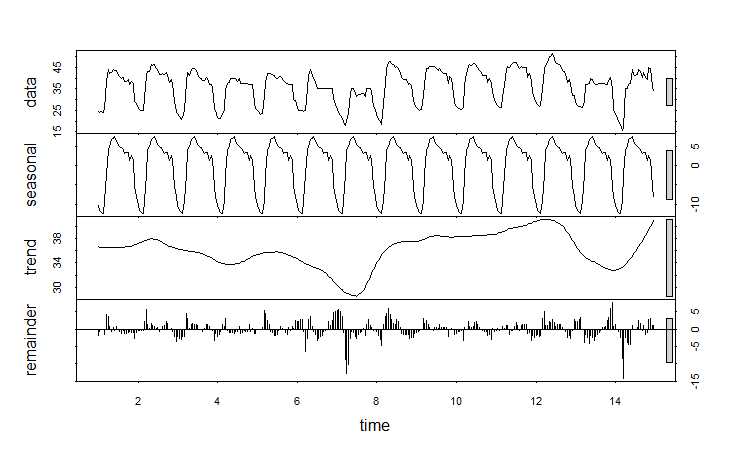
\includegraphics[width=1.00\textwidth]{figures/forecasting/stl_decomposition_July_2014.png}
	\caption{STL decomposition of hourly day ahead time series, Nord Pool Spot, Helsinki from July 7th to July 21st in 2014}	
	\label{fig:stl_decomposition_July_2014}
\end{figure}

The plot consists of four rows with each row containing a different time series component. 
The first row shows the original time series with hourly prices over a time period of two weeks. There are evident daily and weekly seasonal periods visible in the time series. Daily seasonality can be observed by the repetitive pattern of highs and lows over each day whereas weekly seasonality is evident due to the recognizable decline of prices towards the end of each week. 

The second row represents the extracted daily seasonal component which depicts the daily variation in prices. STL is only capable of extracting a single seasonality pattern. In case both daily and weekly seasonal periods should be extracted a BATS or TBATS model can be used (these models are discussed later in this section). 

In the third row the trend component is displayed. It shows a seemingly repetitive pattern over one week, which denotes the weekly seasonal period observable from the original time series. 

Finally in the last row the remaining irregular component is shown which contains all remaining variations in the time series. 

The grey bars at the right hand side of each plot aim to provide a relative comparison of scales over all plots, i.e.~the height of the bars show the same value range in different scales. Thus the whole value range of the trend component is equivalent with the value range of about one third of the original time series. 




\subsection{Forecast models}

Different statistical forecast models have been chosen to be investigated on a large scale. The selection of forecast models includes simpler models such as Simple Exponential Smoothing and more advanced models such as ARIMA and TBATS and variants thereof. The purpose of the evaluation is to provide insights into the performance of different forecast models when applied to electricity price time series. 

\subsubsection{Mean forecast}

The mean forecast is a simple model based on previous observations of a time series. It calculates the mean over a training data set and uses this mean as forecast for all future values \cite{hyndman2012forecasting}. 

It can be formally defined as in equation \ref{eq:mean_forecast}

%\begin{equation}
%\hat{Y}_{t+i} = Y_t
%\label{eq:naive_forecast}
%\end{equation}

\begin{equation}
\hat{y}_{T+h|T} = \frac{1}{T} \sum_{i=1}^T y_i
\label{eq:mean_forecast}
\end{equation}

where $T$ denotes the number of observations in the training dataset, $y_i$ denote historical values and $\hat{y}_{T+h|T}$ denotes a forecast of $h$ values into the future beginning at the value of $y_T$. 

Even though the mean forecast only includes simple calculations it can be effective to forecast random or near random time series or time series that exhibit strong volatility. As it is the simplest of the proposed models it should serve as a baseline model to which other models' performance can be compared. 

\subsubsection{Simple Exponential Smoothing}

The Simple Exponential Smoothing model (SES) belongs to the category of exponential smoothing models which calculate the weighted average over historical observations where weights are exponentially decreased for observations in the past. 

As the name implies this model is the simplest of exponential smoothing models which is designed to provide forecast for time series without trend or seasonal components. Similar to the mean forecast model past values of a time series are processed but with given weights that decrease exponentially over time \cite{hyndman2012forecasting,weron2007modeling}. 

The corresponding formula is depicted in Equation \ref{eq:ses_forecast} 

\begin{equation}
\hat{y}_{T+1|T} = \sum_{i=0}^{T-1} \alpha (1 - \alpha)^i y_{T-i}
\label{eq:ses_forecast}
\end{equation}

where $\alpha$ with $0 \le \alpha \le 1$ denotes the smoothing parameter that determines the influence of past observations through setting the corresponding weights. Thus by modifying values of $\alpha$ the resulting impact of past values to forecasted values can be defined. 

\subsubsection{Holt's Exponential Smoothing}

Holt's Exponential Smoothing (Holt's ES) is a linear trend method which extends Simple Exponential Smoothing by including trends in the model generation process \cite{hyndman2012forecasting}. The model consists of two separately modeled components which are level and trend components. These are combined to obtain forecasts for a given time series. It can be formalized by the following equations:

\begin{align}
 \hat{y}_{t+h|t} &= l_t + h b_t \label{eq:holts_forecast} \\
 l_t &= \alpha y_t + (1 - \alpha) (l_{t-1} + b_{t-1})\label{eq:holts_level_component} \\
 b_t &= \beta (l_t - l_{t-1}) + (1 - \beta) b_{t-1}\label{eq:holts_trend_component}
\end{align}

Equation \ref{eq:holts_forecast} denotes the forecast value $\hat{y}_{t+h|t}$ which is forecasted $h$ steps into the future beginning from time stamp $t$. It consists of a combination of the level $l_t$ at time $t$ and the trend $b_t$ at time $t$ continued over the next $h$ time intervals. 

The level component is described in Equation \ref{eq:holts_level_component} which denotes a linear combination of the actual value $y_t$ at time $t$ and the level forecast constructed from previous time stamp's level $l_{t-1}$ and trend $b_{t-1}$ components. 

Equation \ref{eq:holts_trend_component} depicts the trend component which is a linear combination of the difference of the current and previous levels ($l_t, l_{t-1}$) and the estimated trend component $b_{t-1}$ from the previous point in time. 

$\alpha$ and $\beta$ exhibit characteristics $0 \le \alpha \le 1$ and $0 \le \beta \le 1$ and denote the smoothing parameters for the level and trend components, respectively.

\subsubsection{Seasonal HoltWinter's model}

The Seasonal HoltWinter's model is the first of the discussed models which is capable of modeling seasonality in the dataset. It further extends the capabilities of the SES and Holt's ES models by an additional seasonal component. Thus besides the level and trend components $l_t$ and $b_t$ a seasonal component $s_t$ is introduced, with smoothing parameters $\alpha, \beta, \gamma$, respectively \cite{hyndman2012forecasting}. 

The corresponding equations are defined as

\begin{align}
 \hat{y}_{t+h|t} &= l_t + h b_t + s_{t-m+h_m^+} \label{eq:holtwinter_forecast} \\
 l_t &= \alpha (y_t - s_{t-m}) + (1 - \alpha) (l_{t-1} + b_{t-1})\label{eq:holtwinter_forecast_level_component} \\
 b_t &= \beta (l_t - l_{t-1}) + (1 - \beta) b_{t-1}\label{eq:holtwinter_forecast_trend_component} \\
 s_t &= \gamma (y_t - l_{t-1} - b_{t-1}) + (1 - \gamma) s_{t-m}\label{eq:holtwinter_forecast_seasonal_component}
\end{align}

where $m$ denotes the period of seasonality (e.g.~$m=12$ for monthly data when one year is the base unit) and $h_m^+ = \left\lfloor (h-1) \mod m\right\rfloor + 1$ represents the additional number of steps ahead required to model the corresponding seasonal period $m$. Therefore $s_{t-m+h_m^+}$ denotes the previously occurred seasonal period which is added to the forecast equation in Equation \ref{eq:holtwinter_forecast}. 

The level component in Equation \ref{eq:holtwinter_forecast_level_component} is adjusted by the level of the last occurred seasonal period $s_{t-m}$ to consider seasonal differences. The equation for the trend component $b_t$ is taken directly from the one of Holt's ES in Equation \ref{eq:holts_trend_component} whereas the seasonal component is defined in Equation \ref{eq:holtwinter_forecast_seasonal_component}. 

The seasonal component is denoted as a weighted sum of the current value $y_t$ substracted by previous level and trend components and the value of the seasonal component exactly $m$ periods before. 

The smoothing parameters $\alpha, \beta$ and $\gamma$ are estimated by minimizing the squared one-step prediction error to appropriately weigh the different components to yield best results \cite{r2016language}. 


\subsubsection{ARIMA models}

ARIMA models or Auto Regressive Integrated Moving Average models are highly adjustable time series models that can incorporate a number of features from the dataset. They are capable of modeling correlations in the data as well as provide a smoothing method to dampen the impact of extreme outliers. 

ARIMA models may consist of both autoregressive (AR) and moving average (MA) terms to accurately model the underlying dataset \cite{hyndman2012forecasting,weron2007modeling}. 

\paragraph{AR model} The autoregressive component is used to model dependencies in the data such that correlations within the dataset are reduced. It is defined as a weighted sum of past values of an observation. An AR(p) model is shown in Equation \ref{eq:ar_component}.

\begin{equation}
	y_t = c + \sum_{i=1}^p \phi_i y_{t-i} + e_t
\label{eq:ar_component}
\end{equation}

where $y_t$ is modeled as the sum of the past $p$ values of $y$ plus an additional error component $e_t$ and a constant $c$. AR coefficients $\phi_1,\ldots,\phi_p$ are used to weight past observations and need to be estimated in the model generation process. 

\paragraph{MA model} The moving average component models a time series as a moving average of past error terms. Equation \ref{eq:ma_component} gives the formal definition: 

\begin{equation}
	y_t = c + e_t + \sum_{i=1}^q \theta_i e_{t-i}
\label{eq:ma_component}
\end{equation}

where $e_t$ denotes the forecast error at time $t$ and the error terms are weighted by MA coefficients $\theta_1,\ldots,\theta_q$.

\paragraph{ARIMA model} An ARIMA model consist of both AR and MA terms. In addition ARIMA models are able to model non-stationary time series by applying differencing operations to the dataset. ARIMA(p,d,q) denotes a model consisting of $p$ number of AR terms, $q$ MA terms and $d$ number of differences. 
It can be described as the sum of AR and MA terms:

\begin{equation}
	y_t = \sum_{i=1}^p \phi_i y_{t-i} + \sum_{i=1}^q \theta_i e_{t-i} + e_t + c
\label{eq:arima_model}
\end{equation}

When applying the model the possible applied differences during data preprocessing are reversed by integrating the results which refers to the \textit{Integrating} part of the model. 

ARIMA models can be enhanced to model seasonal periods which are defined as ARIMA (p,d,q)(P,D,Q)\textsubscript{m} also denoted as SARIMA models. 
In addition to non-seasonal parameters $p, d$ and $q$ the seasonal parameters $P$, $D$ and $Q$ denote the seasonal AR, differencing and MA components, respectively. 



\subsubsection{BATS and TBATS models}

Multiple seasonal periods can be applied by models such as BATS and TBATS \cite{r2016language}. This can be done by applying a BATS or TBATS model to the time series, identifying different seasonal and trend components and modeling each component separately \cite{de2011forecasting}. 

Both BATS and TBATS models are able to handle multiple seasonalities in the data, i.e.~considering both daily and weekly seasonal periods where TBATS models are capable of modeling non-integer periods as well (e.g.~365.25 for annual seasonality). 

\paragraph{BATS model} BATS stands for Box-Cox transform, ARMA errors, Trend, and Seasonal components. TBATS can then be regarded as the trigonometric version of BATS. 

The definition of BATS is outlined in the following equations: 


\begin{equation}
	y_t^{(\omega)} = 
	\begin{cases}
		\frac{y_t^\omega - 1}{\omega}, & \omega \neq 0 \\
		\log y_t, & \omega = 0
	\end{cases}
\end{equation}


%\begin{equation}
	%y_t^{(\omega)} = 
	%\begin{cases}
		%\frac{y_t^\omega - 1}{\omega}, & \text{if}\ a=1 \\
		%\log y_t, & \text{otherwise}
	%\end{cases}
%\end{equation}


\begin{align}
	y_t^{(\omega)} &= l_{t-1} + \phi b_{t-1} + \sum_{i=1}^T s_{t-m_i}^{(i)} + d_t\label{eq:bats_model} \\
	l_t &= l_{t-1} + \phi b_{t-1} + \alpha d_t \\
	b_t &= (1 - \phi) b + \phi b_{t-1} + \beta d_t \\
	s_t^{(i)} &= s_{t-m_i}^{(i)} + \gamma_i d_t\label{eq:bats_seasonal} \\
	d_t &= \sum_{i=1}^p \Phi_i d_{t-i} + \sum_{i=1}^q \theta_i e_{t-i} + e_t
\end{align}

where $y_t^{(\omega)}$ denotes the Box-Cox transformed value with parameter $\omega$ where $y_t$ is the current value at time $t$ (See also Box-Cox transform in \ref{ssec:box_cox_transformation}). 

$l_t$ describes the level, $b$ denotes the long term trend, $b_t$ represents the trend, $e_t$ is gaussian white noise with zero mean and constant variance and $s_t^{(i)}$ denotes the i-th seasonal component. $\phi$ denotes the damping parameter for the trend and defines the impact of short and long term trends. All of these components are adjusted by a weighted ARMA component $d_t$ and coefficients $\alpha$, $\beta$ and $\gamma$, respectively. 

A BATS model is parameterized by BATS($\omega$,$\phi$,$p$,$q$,$m_1$,\ldots,$m_T$) with the Box-Cox parameter $\omega$, damping parameter $\phi$, ARMA parameters $p$ and $q$ and seasonal periods $m_1,\ldots,m_T$. A double seasonal model (e.g.~daily and weekly) with an AR(1) component can be described as BATS(1,1,1,0,$m_1$,$m_2$) with default Box-Cox and damping parameters. 

\paragraph{TBATS model} As BATS models possibly result in a large number of states and only pure integer seasonal periods may be modeled, the TBATS model has been developed \cite{de2011forecasting}. This model enhances the BATS model with trigonometric expressions:

\begin{align}
	s_t^{(i)} &= \sum_{j=1}^{k_i} s_{j,t}^{(i)}\label{eq:tbats_seasonal} \\
	s_{j,t}^{(i)} &= s_{j,t-1}^{(i)} \cos \lambda_j^{(i)} + s_{j,t-1}^{*(i)} \sin \lambda_j^{(i)} + \gamma_1^{(i)} d_t \\
	s_{j,t}^{*(i)} &= - s_{j,t-1} \sin \lambda_j^{(i)} + s_{j,t-1}^{*(i)} \cos \lambda_j^{(i)} + \gamma_2^{(i)} d_t 
\end{align}

where $s_{j,t}^{(i)}$ describes the stochastic level of the i-th seasonal component and $s_{j,t}^{*(i)}$ represents the stochastic growth in the level of the i-th seasonal component which can be described as the change of value of the seasonal component over a period of time. $k_i$ is the number of harmonics required for the ith seasonal component, $\gamma_1^{(i)}$ and $\gamma_2^{(i)}$ are smoothing parameters and $\lambda_j^{(i)} = \frac{2 \pi j}{m_i}$ the trigonometric parameter which depends on the corresponding seasonal period $m_i$. 

Finally the model can be obtained by replacing $s_t^{(i)}$ in equation \ref{eq:bats_seasonal} by the trigonometric expression in equation \ref{eq:tbats_seasonal} and replacing $s_{t-m_i}^{(i)}$ in equation \ref{eq:bats_model} by $s_{t-1}^{(i)}$. 


\subsection{Box Cox transformation} \label{ssec:box_cox_transformation}

Box cox transformations are used to transform non-normal data to exhibit a normal distribution like behavior \cite{box1964analysis}. Since most statistical time series models (e.g.~ARIMA) require data to have constant variance this technique can be used as a preprocessing step before applying data to forecasting models \cite{nelson1979experience}. 

The formula for box cox transformations is as follows: 


\begin{equation}
	y^{(\lambda)} = 
	\begin{cases}
		\frac{y^\lambda - 1}{\lambda}, & \lambda \neq 0 \\
		\log y, & \lambda = 0
	\end{cases}
	\label{eq:box_cox_transform}
\end{equation}

\begin{equation}
	y^{(\lambda)} = 
	\begin{cases}
		\frac{(y + c)^\lambda - 1}{\lambda}, & \lambda \neq 0 \\
		\log (y + c), & \lambda = 0
	\end{cases}
	\label{eq:box_cox_transform_with_constant}
\end{equation}

where conditions $y > 0$ and $y > -c$ apply to equations \ref{eq:box_cox_transform} and \ref{eq:box_cox_transform_with_constant}, respectively. 

Since the value of $\lambda$ can be less than one $y$ has to be positive and thus a constant term $c > 0$ is required in case $y < 0$ (equation  \ref{eq:box_cox_transform_with_constant}). 

In \cite{nelson1979experience} the autors show that it might not be always possible to transform a series to show a normal distribution and that the application of the procedure can be costly. Still some improvements to forecasts can be achieved by applying Box-Cox transformation to non-normal distributions as a preprocessing step to model generation. 


\subsection{Forecast accuracy measures} \label{ssec:forecast_acc_measures}

Different forecast accuracy methods can be applied to investigate model performance. These methods are based on estimating the overall forecast error for a given model and forecast horizon \cite{hyndman2012forecasting, weron2007modeling}. 

The forecast errors are computed as a function of residuals which are defined as the differences of actual values to forecasts \cite{hyndman2012forecasting}: 

\begin{equation}
	e_i = y_i - \hat{y_i}
\label{eq:residuals}
\end{equation}

where $\hat{y_t}$ denotes the one step ahead forecast based on a series of past values $\{y_1,\ldots,y_{t-1}\}$. 


\subsubsection{Scale-dependent error measures}

Scale dependent errors are absolute error measures depending on the scale of the examined dataset. Therefore when comparing these types of error measures they should be applied to data showing the same scale. 

\paragraph{Mean error}
The mean error (ME) denotes a measure of the mean value of forecast errors over a given period of time. 
It can be seen as indication of the symmetry of the forecast error distribution. 

\begin{equation}
\frac{1}{n} \sum_{i=1}^{n} \hat{y}_i - y_i
\label{eq:acc_me}
\end{equation}

where $n$ is the number of observations, $\hat{y}_i$ is the forecast for observation $i$ and $y_i$ denotes the actual value for observation $i$. 

\paragraph{Mean absolute error}
The mean absolute error (MAE) shows the mean of all absolute errors over the forecast horizon where the absolute error is defined by the absolute difference between a value of the dataset and its forecasted value. The mean absolute error provides a means for retrieving a measure proportional to actual forecast errors. 

\begin{equation}
\frac{1}{n} \sum_{i=1}^{n} |\hat{y}_i - y_i|
\label{eq:acc_mae}
\end{equation}



\paragraph{Root mean squared error}
The root mean squared error (RMSE) takes the root of the sum of the squared forecast errors which puts more emphasis on possible outliers in residual values. 

\begin{equation}
	\sqrt{\frac{1}{n} \sum_{i=1}^{n} (\hat{y}_i - y_i)^2}
\label{eq:acc_rmse}
\end{equation}


\subsubsection{Percentage based error measures}

Percentage based error measures have the advantage of providing scale independent measures for comparing forecast errors across different time series. However a significant disadvantage of percentage errors is their inability to handle zero values in time series. Also numerical compuations become unstable when values get closer to zero. 


\paragraph{Mean percentage error}

The mean percentage error (MPE) is dependent on the symmetry of the forecast error distribution as positive and negative value differences might cancel each other out. This can be compared to the mean error which shows the same behavior as a scale dependent measure. 


\begin{equation}
\frac{1}{n} \sum_{i=1}^{n} \frac{\hat{y}_i - y_i}{y_i}
\label{eq:acc_mpe}
\end{equation}



\paragraph{Mean absolute percentage error}

The mean absolute percentage error (MAPE) shows similar to the mean absolute error the mean of all absolute errors but as percentage error relative to the corresponding actual value. 

\begin{equation}
\frac{1}{n} \sum_{i=1}^{n} \left|\frac{\hat{y}_i - y_i}{y_i}\right|
\label{eq:acc_mape}
\end{equation}




\section{Model generation} \label{sec:model_generation}

In this section the procedure of generating an ARIMA model is described. Since ARIMA models are classical time series models which showed reasonable results in energy price forecasting \cite{aggarwal2009electricity,weron2005forecasting} they have been investigated in detail to provide a better understanding of the model generation process. 

In addition to the well known Box Jenkins approach (see section \ref{ssec:arima_models_to_predict_next_day_prices}) a custom model selection process is proposed for manual ARIMA model selection \cite{hyndman2012forecasting}. This process is outlined in Figure \ref{fig:manual_arima_forecasting_procedure}.

\begin{figure}[htbp]
	\centering
		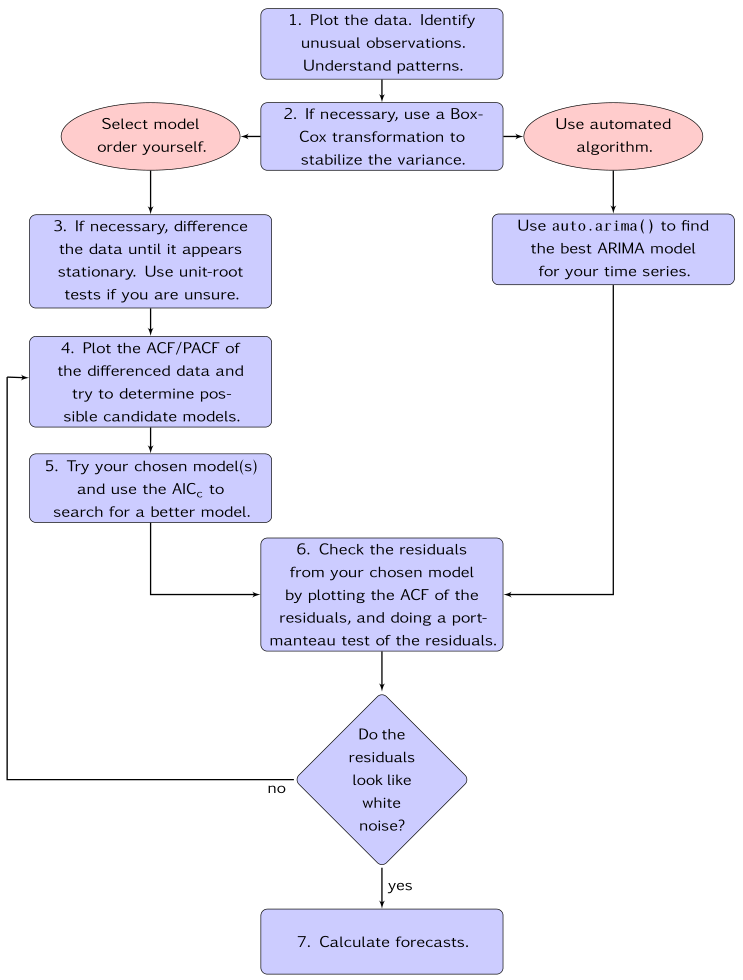
\includegraphics[width=0.70\textwidth]{figures/forecasting/manual_arima_forecasting_procedure.png}
	\caption{Manual ARIMA model generation process \cite{hyndman2012forecasting}}
	\label{fig:manual_arima_forecasting_procedure}
\end{figure}

In this case a manual model generation process is conducted. The data based on which a model will be generated together with diagnostic plots (ACF, PACF) is shown in Figure \ref{fig:tsdiag_prices_acf_pacf}. 

\begin{figure}[htbp]
	\centering
		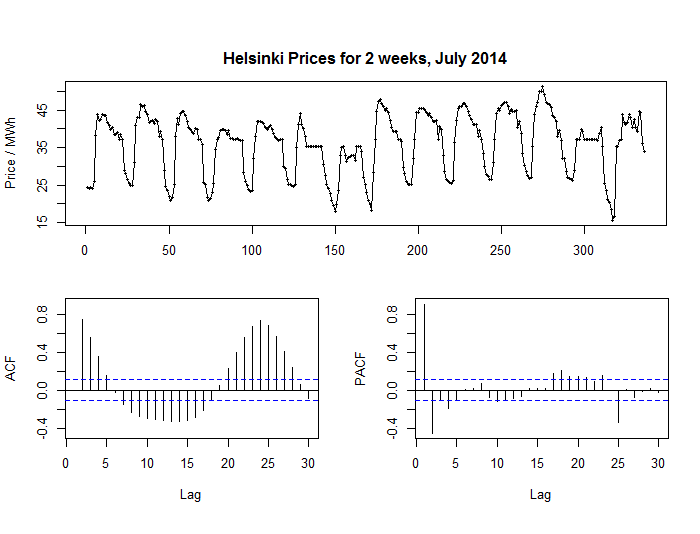
\includegraphics[width=0.95\textwidth]{figures/forecasting/tsdiag_prices_acf_pacf.png}
	\caption{Two weeks of hourly day ahead prices with ACF and PACF plots (Nord Pool Spot, Helsinki from July 7th to July 21st in 2014)}
	\label{fig:tsdiag_prices_acf_pacf}
\end{figure}

The dataset consists of two weeks of hourly day ahead prices amounting to a total of 336 hours. Figure \ref{fig:tsdiag_prices_acf_pacf} shows three plots, at the top a time series plot showing the energy price time series is depicted, on the bottom left an autocorrelation plot (ACF) is shown and on the bottom right a partial autocorrelation plot (PACF) is printed. 
As already discussed in section \ref{ssec:seasonal_decomposition} this data exhibits daily and weekly seasonality which is clearly visible on the time series plot. 

As ARIMA models require data to be stationary (i.e.~it exhibits no trend or seasonality) the proposed method to transform a series into a stationary series is to apply one or more levels of differencing or seasonal differencing. The resulting residuals of the model should show no autocorrelations and should exhibit a zero mean \cite{hyndman2012forecasting}. Ideally residuals have constant variance and exhibit a normal distribution as well. 

ACF and PACF plots are diagnostic plots to examine correlations within the dataset \cite{nist2012handbook,nau2016statistical}. 
Both ACF and PACF plots display individual lags on the x-coordinate while on the y-coordinate the values of the autocorrelation and partial autocorrelation functions are displayed for ACF and PACF plots, respectively. The dashed blue lines denote the 95\% confidence interval for white noise, i.e.~lag values contained within this interval do not reject the white noise hypothesis. 
Values exceeding the confidence bounds are "`significant"' regarding correlations in the data. 
%However 1 in 20 lags is allowed to exceed the significance bounds without violating the white noise assumption. 

The ACF plot displays the ``coefficients of correlation between a time series and lags of itself'' whereas the PACF plot shows the ``partial correlation coefficients between the series and lags of itself'' \cite{nau2016statistical}. 
Correlation coefficients for autocorrelations are said to be interdependent which means that the value of an autocorrelation at lag $h$ depends on correlations of all previous lags $1,\ldots,h-1$. In contrast, partial autocorrelations only include correlations specific to lag $h$ without considering correlations at lower order lags. 

According to the model generation process in Figure \ref{fig:manual_arima_forecasting_procedure} data should be differenced if necessary to make the series stationary. In this case a seasonal difference might be appropriate due to the obvious seasonality in the time series. 

The ACF plot above shows a decay of significant autocorrelations whereas the PACF plot depicts several significant spikes with most significant ones at lags 2 and 25. 
As the spike at lag 25 in the PACF plot is close to the assumed seasonal period of 24 this may suggest adding a seasonal AR(1) term with a period of 24. The peak value at lag 24 in the ACF plot may be another indicator of seasonal correlation.
Therefore, the suggested intermediate ARIMA model is ARIMA(0,0,0)(1,1,0)[24] with a seasonal AR term and one level of seasonal differencing with a period of 24. 

The resulting model residuals are depicted in Figure \ref{fig:residuals_arima_000_110}. 

\begin{figure}[htbp]
	\centering
		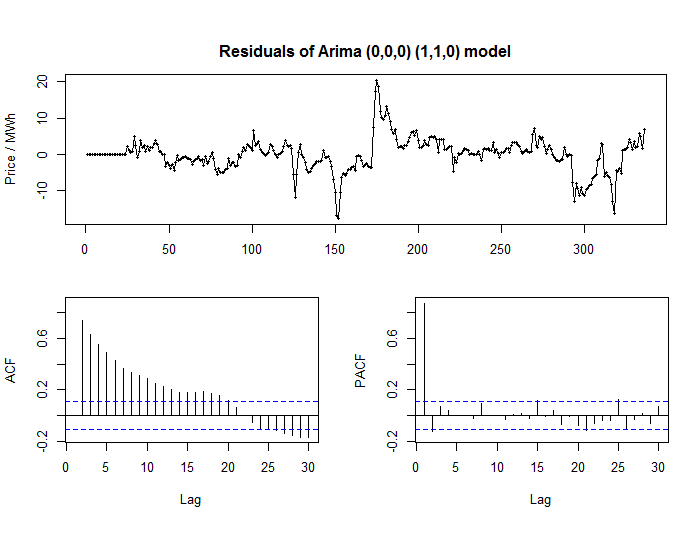
\includegraphics[width=0.95\textwidth]{figures/forecasting/residuals_arima_000_110.png}
	\caption{Intermediate ARIMA(0,0,0)(1,1,0)[24] model with seasonal difference}
	\label{fig:residuals_arima_000_110}
\end{figure}

Figure \ref{fig:residuals_arima_000_110} depicts residuals with removed hourly seasonality and zero mean. However the series can not be regarded as stationary as significant deviations exist from the mean in the time series. Apart from the weekly seasonality further correlations can be identified. 

According to \cite{nau2016statistical} a cut-off (rapid decrease of correlation values) at the PACF plot indicates adding an AR term with an order corresponding to the number of the last significant lag of this occurrence. Conversely a cut-off at the ACF plot indicates the addition of a MA term with the number of the last significant lag in the ACF plot. 

Since Figure \ref{fig:residuals_arima_000_110} shows a slow decay in the ACF and a small but significant coefficient at lag 2 in the PACF we recognize a cut-off at this lag in the PACF and add a (non-seasonal) AR(2) term to the model. 
Thus the resulting model is ARIMA(2,0,0)(1,1,0)[24] which is shown in Figure \ref{fig:residuals_arima_200_110}. 

\begin{figure}[htbp]
	\centering
		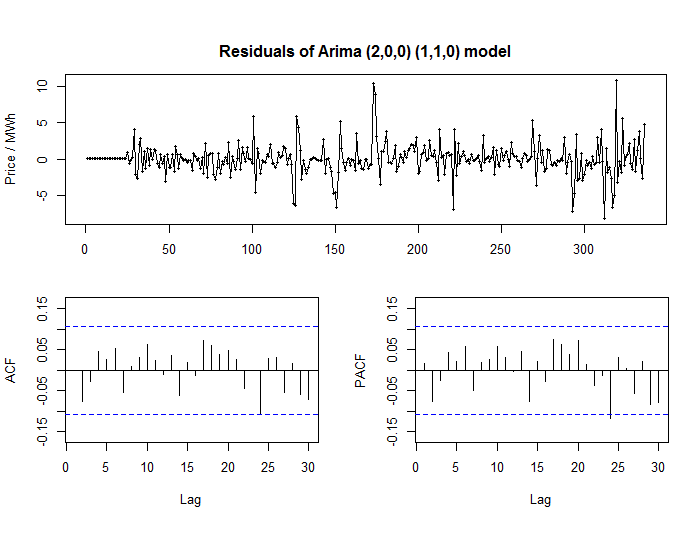
\includegraphics[width=0.95\textwidth]{figures/forecasting/residuals_arima_200_110.png}
	\caption{Residuals of ARIMA(2,0,0)(1,1,0)[24]}
	\label{fig:residuals_arima_200_110}
\end{figure}

The time series of residuals above can be assumed to be stationary as no significant deviations from the mean are visible. 

There is only one significant spike at lag 24 remaining which might indicate still some seasonal information in the data, however it could be as well regarded as outlier as 1 in 20 spikes is said to be significant by chance alone \cite{hyndman2012forecasting}. 


%
%The autocorrelation function determines the existence or non-existence of correlation between lagged variables within a time series \cite{nist2012handbook}. 
%That is, the correlation between a point in the time series to another point in the same time series is calculated where the gap between the two points is fixed by the given lag (hence the name \textit{auto}-correlation). 
%
%The autocorrelation function is defined as the autocorrelation coefficient $R_h$ (equation \ref{eq:autocorr_coeff})
%
%\begin{equation}
%R_h = \frac{C_h}{C_0}
%\label{eq:autocorr_coeff}
%\end{equation}
%
%
%where $C_h$ denotes the autocovariance function and $C_0$ defines the variance function 
%(see equations \ref{eq:autocov_func} and \ref{eq:variance_func}). 
%
%
%\begin{equation}
%C_h = \frac{1}{N} \sum\limits_{t=1}^{N-h} (Y_t - \bar{Y}) (Y_{t+h} - \bar{Y})
%\label{eq:autocov_func}
%\end{equation}
%
%
%\begin{equation}
%C_0 = \frac{1}{N} \sum\limits_{t=1}^{N} (Y_t - \bar{Y})^2
%\label{eq:variance_func}
%\end{equation}
%
%with $\bar{Y}$ denoting the mean of the series, $N$ defines the sample size, $Y_t$ the observation at time $t$ and $Y_{t+h}$ the observation $h$ steps ahead from $t$. 
%The autocovariance function determines the mean of covariance between variables with fixed lag $h$ while the variance function determines the mean variance over all timestamps $N$. 



\subsection{Model validation}



The corrected Akaike Information Criterion (AICc) is a well known goodness of fit measure for stochastic models \cite{weron2007modeling}. It provides a relative quality measure for models such that models with lower AICc values are assumed to better capture the characteristics of the underlying data. 
Equation \ref{eq:aicc_test} defines the metric. 

\begin{equation}
	AICc = -2 \log \mathcal{L} + \frac{2dn}{n - d - 1}
\label{eq:aicc_test}
\end{equation}

with $\log \mathcal{L}$ being the log-likelihood, $d$ the model size (number of parameters) and $n$ denotes the sample size. Note that the model size $d$ is present in order to penalize models having too many parameters. The log-likelihood function estimates how well the model fits the data. 

After a model has been chosen by evaluating the AICc value the model residuals should be checked for existing correlations. As shown in the last section this can be done by verifying the ACF and PACF plots but tests are available for automated testing against randomness \cite{weron2007modeling,hyndman2012forecasting}. 

One of these tests is the Ljung Box test which tests a given number of autocorrelations if they fall outside the significance bounds \cite{weron2007modeling}. The test is defined in Equation \ref{eq:ljung_box_test}. 

%for probability of showing non-white noise properties 
\begin{equation}
	Q = n(n + 2) \sum_{j=1}^{h} \frac{\hat{\rho}^2 (j)}{n - j}
\label{eq:ljung_box_test}
\end{equation}

with $n$ as the sample size, $h$ as number of lags and $\hat{\rho}^2 (j)$ as the squared autocorrelation at lag $j$. 
Its distribution can be approximated by the $\chi^2$ distribution with $h$ degrees of freedom. The white noise hypothesis is rejected if $Q > \chi_{1-\alpha}^2 (h)$ with a defined significance level $\alpha$ with $\chi_{1-\alpha}^2$ being the $(1 - \alpha)$ quantile of the $\chi^2$ distribution with $h$ degrees of freedom. 


\subsection{Model evaluation} \label{ssec:model_evaluation}

In order to assess the quality and goodness of fit of the models generated in section \ref{sec:model_generation} they are validated and compared to a model generated by an automatic model generation procedure. 

In addition to the manual model selection procedure shown in the last section automatic model generation procedures exist to detect the model with best goodness of fit parameters by iterating over a set of candidate models. 

For generating ARIMA models the \textit{auto.arima} function may be used \cite{hyndman2012forecasting,r2016language}. 

It is defined by the following steps \cite{hyndman2012forecasting}: 

\begin{enumerate}
	\item Determine the number of differences $d$ by applying a unit root test (e.g.~KPSS test).
	\item A set of candidate models is generated starting with the following models: 
				
				ARIMA(2,d,2) \\
				ARIMA(0,d,0) \\
				ARIMA(1,d,0) \\
				ARIMA(0,d,1) 
				
				Model parameters $p$ and $q$ are modified by adding $\pm 1$ where the best model is set as reference. 
				Repeat the last line until no model with a lower AICc value can be found. 

\end{enumerate}

A model has been generated using auto.arima based on the same data as used for manual model selection in section \ref{sec:model_generation}. 
The resulting models with corresponding model parameters are outlined in table \ref{tab:model_names_and_parameters}. 

\begin{table}[ht]
\centering
\begin{tabular}{l|l}
 Model Name & Model Parameters \\ 
  \hline
	Intermediate Model	& ARIMA(0,0,0)(1,1,0)[24] \\ 
	Final Model 				& ARIMA(2,0,0)(1,1,0)[24] \\ 
	Automatic Model 		& ARIMA(2,0,3)(1,0,2)[24] \\ 
\end{tabular}
\caption{Model names and parameters}
\label{tab:model_names_and_parameters}
\end{table}

AICc and Ljung Box values have been calculated for each model defined above. For Ljung Box tests a 95\% confidence interval has been used
such that resulting p-values greater than 0.05 indicate white noise properties of the residuals. Thus a high Ljung Box test value gives 
high probability of a series resembling white noise. 

The AICc and Ljung Box values are outlined in table \ref{tab:model_aicc_and_ljung_box_values}. 

\begin{table}[ht]
\centering
\begin{tabular}{r|r|r|r}
 & Intermediate Model & Final Model & Automatic Model \\ 
  \hline
	AICc 			& 1868.01 & \textbf{1400.22} & 1457.26 \\ 
  Ljung Box & < 2.2e-16 & 0.1523 & \textbf{0.9927} \\ 
\end{tabular}
\caption{AICc and Ljung Box values}
\label{tab:model_aicc_and_ljung_box_values}
\end{table}

Results show that it is possible for manually selected models to outperform automatically generated models, i.e.~the Final Model shows a lower AICc value than the Automatic Model. This is presumably due to the manual model using explicit seasonal differencing which the automatic nodel does not use. However the Ljung Box test values indicate a different result where the Automatic Model results in a higher p-value and thus exhibits less correlations than the Final Model. As both models exceed the significance bounds of 0.05 this is only of minor importance as both exhibit white noise characteristics. If in doubt the AICc value should be given precedence over Ljung Box test results. 

\section{Model selection algorithm} \label{sec:model_selection_algorithm}

An automated model selection algorithm has been implemented to provide aid in finding suitable ARIMA models for a given training dataset. 
The process consists of several data preprocessing steps with generation and comparison of different ARIMA models and model evaluation based on a weighted function of AICc and Ljung Box test values. 

The model selection algorithm consists of three separate functions each contributing a different part to model generation. These functions are \textit{GenerateArimaModel} as the base function for model generation, \textit{AutomatedBoxTest} for determining the right parameters for the Ljung Box tests and \textit{SeasonalPeriods} for estimation of possibly existing seasonal periods within the data. 

%They will be referred to each other as soon as they are called. 

\subsection{Function GenerateArimaModel}

\begin{enumerate}
	\item Get trainingdata
	
	\begin{enumerate}
		\item Read time series of energy prices from given location
		\item Define training period by start and end date
	\end{enumerate}
	\item Determine seasonality
	
	\begin{enumerate}
		\item Call \textit{SeaonalPeriods} to retrieve seasonal periods from the data
	\end{enumerate}
	
	\item Create time series objects
	
	\begin{enumerate}
		\item For each seasonal period found create a time series object based on that period
	\end{enumerate}
	
	\item Calculate the Box-Cox transformation parameters
	
	\begin{enumerate}
		\item Compute the Box Cox parameters for each of the created time series objects
	\end{enumerate}
	
	\item Create models
	
	\begin{enumerate}
		\item Create model(s) without BoxCox transformation
		
		\begin{enumerate}
			\item Generate model with auto.arima for each of the created time series objects 
		\end{enumerate}
		
		\item Create model(s) with BoxCox transformation
		
		\begin{enumerate}
			\item Generate model with auto.arima and previously defined lambda (Box-Cox) parameter for each of the created time series objects if Box-Cox parameter is not equal to 1 (then it would have no effect)
		
		\end{enumerate}
		
	\end{enumerate}
	
	\item Execute Ljung Box test for each of the models
	
	\begin{enumerate}
		\item Call \textit{AutomatedBoxTest} to retrieve the Ljung Box p-values for each model
	\end{enumerate}
	
	\item Saving models, boxtests, AICc values and p-values in vectors
	
	\item Model Evaluation

	\begin{enumerate}
		
		\item Check model goodness of fit via AICc value comparison
		
		\begin{enumerate}
			\item $p_{aicc_i} = \frac{1}{| AIC_{min} - AIC_i | + 2}$
			%\item p_aicc = 1 / (abs(AICmin – AIC(i)) + 2)
			\item ``+2'' -> moderate the decrease of values due to the inverse function
		\end{enumerate}
		
		\item Compare p-values of Ljung Box tests to check residual characteristics
		
		\begin{enumerate}
			\item p-values range from 0 to 1 -> determine difference in relation to full range
			\item $p_{ljung} = \frac{p_{value} - 0.05}{1 - 0.05}$
		\end{enumerate}
		
	\end{enumerate}

	\item Model selection

	\begin{enumerate}
		\item Calculate weighted result based on goodness of fit values with user defined weights
		\item $F_i = w_{aicc_i} p_{aicc_i} + w_{ljung_i} p_{ljung_i}$ for each model $i \in M$
	\end{enumerate}
	
	\item Return model with the highest goodness of fit value $F_i$

\end{enumerate}


\subsection{SeasonalPeriods}

	\begin{enumerate}
		\item If target period is specified and enforced
		
		\begin{enumerate}
			\item return a list of (targetPeriod, defaultPeriod) 
		\end{enumerate}
		
		\item Else 
		
		\begin{enumerate}
			\item Get the x most frequent periods sorted by number of occurrences descending, where x is a user defined number (apply periodogram)
			\item If a max period limit has been specified, discard any periods above this limit
			\item If the number of occurrences of a period falls below the white noise threshold, discard the period
			
			\item If the target period is specified and has been found
			
			\begin{enumerate}
				\item return a list of (targetPeriod, defaultPeriod) 
			\end{enumerate}
			
			\item Otherwise
			
			\begin{enumerate}
				\item add the defaultPeriod (=1) to the list of periods and return the list
			\end{enumerate}
		\end{enumerate}
	\end{enumerate}


\subsection{AutomatedBoxTest}

\begin{enumerate}
	\item Determine the most suitable value for the lag based on the sample size and 
	whether seasonal periods are existing in the dataset. 
	
	\begin{enumerate}
		\item The following rules of thumb have been established to determine a suitable value for the lag of the test \cite{hyndman2014blog}: 
		
		\begin{enumerate}
			\item for non-seasonal time series a lag value of $h=min(10,T/5)$ should be used
			\item for seasonal time series a lag value of $h=min(2m,T/5)$ should be used,
				where $T$ denotes the sample size and $m$ the seasonal period
		\end{enumerate}
		
		\item The number of determined lags is reduced by the number of parameters in the model
		
		\item The box test is executed and result is returned
	\end{enumerate}
	
\end{enumerate}


\subsection{Discussion}

The core of the model selection algorithm are steps 8 and 9 of Function GenerateArimaModel where relative measures for both AICc and Ljung Box values have been developed to be able to integrate them into a weighted function. Thus it is possible to define weights to define the impact of each validation measure on forecast model selection. 
As mentionend before (Section \ref{ssec:model_evaluation}) AICc value results should in general be given precedence over Ljung Box values since AICc values are considered more stable. 

Another thing to note is the so called \textit{target period} in function \textit{SeasonalPeriods}. This is a user estimated period which is assumed to be contained in the dataset. If it is found it is given precedence over other periods returned. There is also the possibility of ``enforcing'' the period in which case it is taken without calculating other periods. 





\section{R / Java Simulation Framework} \label{sec:r_java_simulation_framework}

The R / Java Simulation Framework is responsible for preparation and execution of a large scale simulation of generating and evaluating forecast models over an extended period of time. In this section the architecture and implementation of the simulation framework is presented as well as the interfaces existing between R and Java. 


\subsection{Architecture of the simulation framework}

The framework consists of a Java application server connected to a separately running R server on which R commands are executed. R is a statistical program which is able to model complex statistical functions and includes a considerable amount of statistical packages \cite{r2016project}. It became the de-facto standard for stochastic processing and is available free of charge as well as for various platforms. 

The Java application server has been set up as WildFly 8 \cite{red2016wildfly} with Java Enterprise Edition 7 \cite{oracle2016java} and an Oracle Database \cite{oracle2016database} which provides a scalable architecture including the possibility for modeling web service interfaces. 

In this work a collection of web services has been set up for simple access of data for external applications. This can be used e.g.~by the cloud simulator outlined in section \ref{sec:architecture_of_simulation_framework}. The Java application server wraps methods for retrieval and storage of energy price data, forecast model generation and large scale simulations. It utilizes R for complex statistical processing which is included into advanced methods for simulations and model generation. 

\subsubsection{Class diagram}

In order to visualize the most important entities of the framework a class diagram is outlined in Figure \ref{fig:EPMA_class_diagram}.

A basic entity for energy price retrieval is the \textit{Resource} which wraps the retrieved contents of an energy price source. Data retrieval happens over a generic \textit{DataFetch} interface which is able to fetch data from an URL (e.g.~web service) or directly from a file. The parsing of the energy price data is achieved by a generic \textit{Parser} interface which can be implemented by Parsers for different file types (currently XLS and CSV). 

A \textit{ResourceType} stores a reference to a specific DataFetch and Parser implementation. As source types and formats of energy data will be different for each energy market at least one DataFetch and Parser implementation has to be provided for each market. The \textit{ResourceManager} keeps track of all resources associated with a registered energy market. It is implemented by resource managers for day ahead and real time markets, respectively. 

The \textit{MarketData} entity handles all the logic necessary for actually retrieving energy price data for a given Resource. It provides methods to retrieve data from registered energy sources and subsequently parsing and importing the data into the database. Instances of MarketData are used by \textit{RTPricesResourceRESTService} and \textit{DAPricesResourceRESTService} that provide web service interfaces for data retrieval. In turn, \textit{RManagerResourceRESTService} utilizes these web services to retrieve energy price data for model generation and forecast simulations. 

\begin{figure}[htbp]
	% used to position the image at the horizontal center of the page
	\hspace*{0.5in}
		% include the graphic rotated by a 90 degree angle and scale to paperwidth and height
		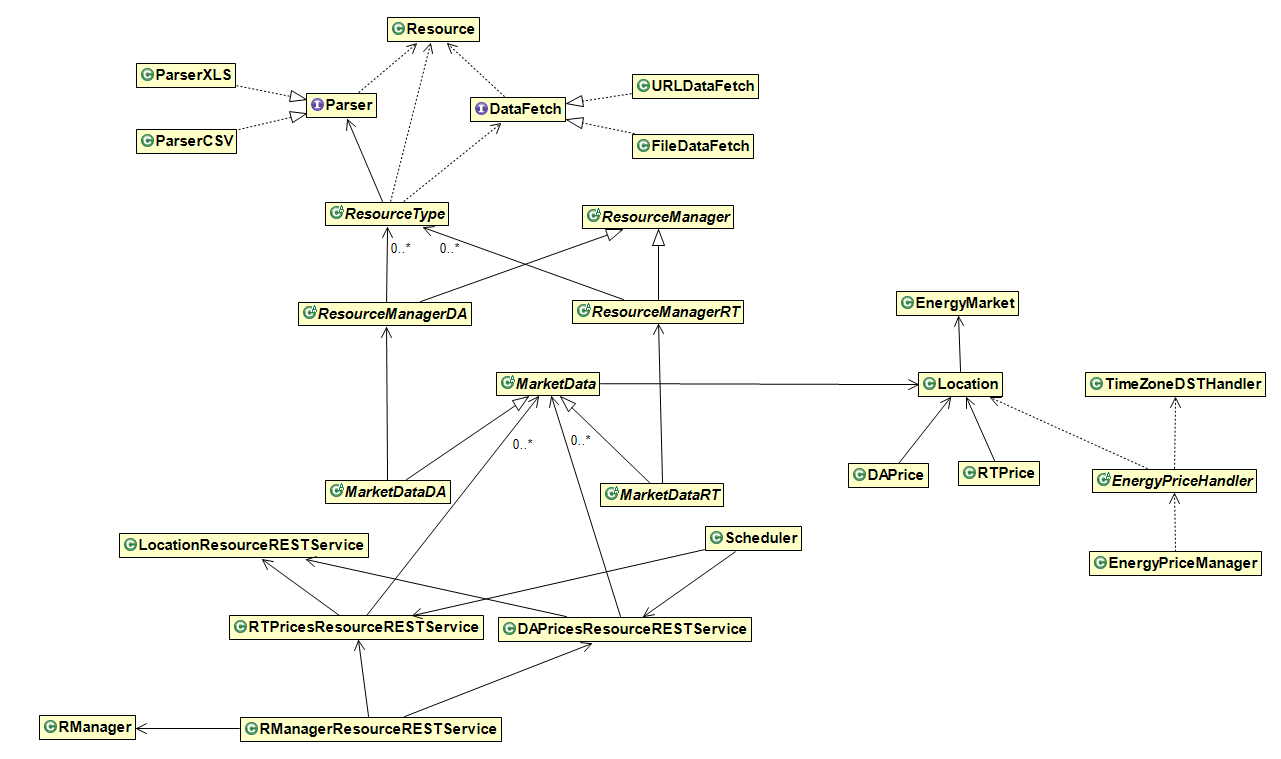
\includegraphics[angle=90,width=\paperheight,height=\paperwidth,keepaspectratio=true]{figures/forecasting/EPMA_class_diagram.png}
	\caption{Class diagram of Energy Price Management Application}
	\label{fig:EPMA_class_diagram}
\end{figure}

The \textit{Scheduler} utilizes Java EE scheduling mechanisms to automatically retrieve energy prices from specific locations at defined time intervals (e.g.~each day at 3 pm). Thus for continuous operation a scheduler can be set up for a location and dates when data should be retrieved regularly from defined interfaces. 

Each MarketData instance stores a reference to a specific \textit{Location} of an \textit{EnergyMarket}. Instances of \textit{DAPrice} and \textit{RTPrice} reference the location from which they were retrieved where these price entities each resemble exactly one energy price entity stored in the database.

Finally the \textit{EnergyPriceHandler} provides a generic interface for parsing energy prices with location specific DST (daylight saving time) changes. This interface is extended by specific implementations of energy markets to manage DST dates. The \textit{TimeZoneDSTHandler} provides a method to retrieve exact DST dates for each location and year. Thus energy prices are stored with dates correctly considering DST changes specific to each location. 

\subsubsection{Web Service interfaces}

The \textit{Energy Price Management Application} (EPMA) on the application server provides different types of web service interfaces. 

Web services are grouped by type: 
%i.e.~management of day ahead prices, real time prices, locations, energy markets and R resources corresponding to classes 

\begin{itemize}
	\item \textit{DAPricesResourceRESTService} for managing day ahead prices
	\item \textit{RTPricesResourceRESTService} for managing real time prices
	\item \textit{LocationResourceRESTService} for managing locations
	\item \textit{EnergyMarketResourceRESTService} for managing energy markets
	\item \textit{RManagerResourceRESTService} for managing R resources
\end{itemize}

Each web service interface is defined by a base path (e.g.~/rtprices), the respective web service name (e.g.~/importall) and mandatory or optional web service parameters. 

%idea: list of all web service methods in the appendix
%
%provide tables with following structure: 
%basepath	web service name		mandatory parameters			optional parameters


%\subsubsection{Energy price data retrieval}



\subsection{R Forecast evaluation}

%fcHorizons <- c("1h","3h","6h","12h","18h","24h","36h","48h","96h","168h")
%accMeasures <- c("ME","RMSE","MAE","MPE","MAPE")
%modelNames <- c("mean","ses","holts","holtwinters","arima","tbats")

The forecast model evaluation discussed in Section \ref{sec:forecast_model_evaluation} is based on implementation of an R function which is called and processed by respective methods on the application server. 

The corresponding R function is named \textit{evaluateModels} and takes energy price data as input separated into a training and test data sets. It generates different forecast models based on the given training set considering possible seasonal periods in the data (see Section \ref{sec:model_selection_algorithm}) and returns aggregated accuracy measures for each model and forecast horizon. 

\subsubsection{Function evaluateModels}

\begin{tabular}{ll}
\textbf{Input:}  & \textit{pricesTraining} - a list of energy prices taken as training data set \\
								 & \textit{pricesTest} - a list of energy prices taken as test data set \\
\textbf{Output:} & \textit{modelList} - a list of models generated within the function \\
								 & \textit{accuracyList} - a list of accuracy measures calculated for each model
\end{tabular}


\begin{lstlisting}[language=R, caption=Function evaluateModels, label={lst:evaluateModelsR}]
evaluateModels <- function(pricesTraining, pricesTest)
{
  period <- getSeasonalPeriod()
  pricesTrainingTs <- generateTimeSeries(pricesTraining, period)
  modelList <- generateModels(Mean,Ses,Holt,HoltWinters, 
	                              Arima,Tbats)						
  accuracyList <- list()
  forecastHorizonList <- (1,3,6,12,18,24,36,48,96,168)
  for( m in modelList ) {
    for( h in forecastHorizonList ) {
      fc <- getForecastForHorizon(m,h)
      accuracyList(m,h) <- getAccuracyMeasures(fc,pricesTest)
    }
  }
  return list(modelList,accuracyList)
}
\end{lstlisting}

In Listing \ref{lst:evaluateModelsR} the function \textit{evaluateModels} is defined. In lines 3 and 4 the most prevailing seasonal period (if any) is determined and 
a time series object is generated based on that period. In line 5 a series of forecast models is generated that are investigated in the algorithm which are Mean forecast model, SES model, Holt (SES with trend), HoltWinters (SES with trend and seasonality), ARIMA (model generation described in Section \ref{sec:model_generation}) and TBATS (seasonal model). 

Line 8 sets a list of forecast horizons in hours, i.e.~forecasts are generated for horizons from 1 up to 168 hours. In line 11 forecasts are produced for each model and forecast horizon separately and in line 12 the generated forecasts are validated by getting accuracy measures for out-of-sample forecasts based on the test data set. 
Line 15 returns a compound object of the list of generated models and accuracy measures. 



\subsection{Java implementation on application server} \label{ssec:java_implementation_on_application_server}

A large scale evaluation of forecasting methods should be conducted where models and corresponding accuracy measures are generated for different training data sets over an extended period of time. 
Thus the application server implements methods for performing customizable forecasting simulations. 

A java method \textit{evaluateModels} in class \textit{RManager} has been implemented which calls the previously introduced R function \textit{evaluateModels} (Listing \ref{lst:evaluateModelsR}) and saves the result in an internal folder on the application server. 
This method is in turn called by an identically named method in \textit{RManagerResourceRESTService} which provides the REST service interfaces to external applications for retrieval of results. 

In order to conduct automated large scale simulations additional methods have been implemented in \textit{RManagerResourceRESTService} to perform customizable simulations. The method \textit{runSimulation} performs a simulation based on a number of parameters. The method signature is depicted in Listing \ref{lst:runSimulation}. 

\begin{minipage}{\linewidth}
\begin{lstlisting}[language=Java, caption=Method runSimulation, label={lst:runSimulation}]
runSimulation(String priceType, Long locationId, 
              String simulationStart, String simulationEnd,
              String trainingPeriod, String testPeriod, String intervalPeriod)
\end{lstlisting}
\end{minipage}

The \textit{priceType} defines whether the simulation should be based on day ahead or real time prices. Accordingly the parameter is set to either ``da'' or ``rt''. The \textit{locationId} expects an Id of a registered location within the application server. The parameter \textit{simulationStart} expects a date time String containing the start date from where the simulation should be started. The parameter \textit{simulationEnd} describes the end date of the simulation as a date time String, respectively. \textit{trainingPeriod} is the training period for which energy prices should be loaded for model generation, \textit{testPeriod} is the test period against which the models are to be tested and \textit{intervalPeriod} denotes the time interval the simulation should be advanced in each step. 

The corresponding web service interface is given in Listing \ref{lst:runSimulationWebService}. 

\begin{minipage}{\linewidth}
\begin{lstlisting}[language=Java, caption=Method runSimulation web service interface, label={lst:runSimulationWebService}]
/r/simulation/{type}/{loc_id}/{simulationStart}/{simulationEnd}/
                {trainingPeriod}/{testPeriod}/{intervalPeriod}
\end{lstlisting}
\end{minipage}

The base path of the web service interface is \textit{/r} which is an indicator for web services that are based on R implementations. The name of the web service is \textit{simulation} and parameters have already been described for Listing \ref{lst:runSimulation}. This method or interface is responsible for executing a single simulation with defined start and end dates, training-, test- and interval periods. 

A common format has been defined to distinguish different periods and intervals. A regular expression for the format could be described as \textit{\textasciicircum\textbackslash d+[hdw]\$}
which is a combination of at least one digit and one of \textit{h}, \textit{d} or \textit{w} which means \textit{hour}, \textit{day} and \textit{week}, respectively. 
Therefore a training period of 2w, 1d or 48h means two weeks, one day or 48 hours. The same holds true for test- and interval periods. 

The method \textit{runSimulation} calls the method \textit{evaluateModels} which performs a single model evaluation for a given training and test period. Its method signature is depicted in Listing \ref{lst:evaluateModels}. 

\begin{minipage}{\linewidth}
\begin{lstlisting}[language=Java, caption=Method evaluateModels, label={lst:evaluateModels}]
evaluateModels(String simulationName, String priceType, Long locationId, 
              String startTraining, String endTraining,
              String startTest, String endTest)
\end{lstlisting}
\end{minipage}

This method is responsible for conducting a model evaluation by calling the respective same-named function on the \textit{RManager}. This method is called for each simulation run triggered by the \textit{runSimulation} method, i.e.~it is called for different training-, test- and interval periods. In order to distinguish different simulations where each simulation is saved in a folder named after the simulation name the simulationName has been normed (Listing \ref{lst:simulationName_definition}): 

\begin{minipage}{\linewidth}
\begin{lstlisting}[caption=Simulation name definition, label={lst:simulationName_definition}]
Definition of the simulation name: 
	
<priceType>_sim_<locationId>_<trainingPeriod>_<testPeriod>_<intervalPeriod>
\end{lstlisting}
\end{minipage}

where \textit{priceType} is the type of energy price (``da'' or ``rt''), \textit{sim} is a delimiter common to all simulations, \textit{locationId} is the id of the location for which to conduct the simulation, \textit{trainingPeriod} is the encoded form of the training period, the same holds true for \textit{testPeriod} and \textit{intervalPeriod}. All parameters are delimited by underscores to clearly distinguish different parameters. 

Therefore a valid simulation name would be \textit{da\_sim\_1\_2w\_1w\_1w} denoting a simulation on day ahead prices for location with Id 1, 2 weeks training period, 1 week test period and 1 week interval period. 

The method \textit{runSimulation} calls the method \textit{evaluateModels} repeatedly over the whole simulation time period (simulation start to simulation end) in intervals specified by the \textit{intervalPeriod} with training and test periods specified by the \textit{trainingPeriod} and \textit{testPeriod} parameters. 

The results of each call of evaluateModels are saved in a separate file under a folder named the same as the simulation. Each file has a naming convention of \textit{<simulationName>\_<start\\Training>} where \textit{startTraining} denotes the start date of the training period for this simulation. 



\section{Forecast model evaluation} \label{sec:forecast_model_evaluation}

A large scale forecast model evaluation is performed over an extended period of time in order to identify models that show good performance across different sets of energy price time series. Different metrics and forecast horizons are investigated for a thorough evaluation of model performance to derive the best model from the simulations. 

Four simulations have been run based on data from four different energy markets, namely \textit{Nord Pool Spot}, \textit{Belpex}, \textit{ISO New England} and \textit{PJM}. A time period of three years of energy price data has been chosen to be able to make a meaningful statement about forecast performance on energy prices. 

For each of these locations three different training periods have been evaluated: two weeks, three weeks and four weeks. The simulations have been run with intervals of 1 week. The (maximum) test period has been set to 1 week as well. 

The resulting simulations according to the defined format in Section \ref{ssec:java_implementation_on_application_server} are outlined in Table \ref{tab:list_of_conducted_forecast_simulations}. Each of these simulations and models are evaluated for five different accuracy measures to get a broader view of the model performances (see also Section \ref{ssec:forecast_acc_measures}): 

\begin{itemize}
	\item Mean error (ME)
	\item Mean absolute error (MAE)
	\item Root mean squared error (RMSE)
	\item Mean percentage error (MPE)
	\item Mean absolute percentage error (MAPE)
\end{itemize}

In addition, each of these error measures has been evaluated for ten different forecast horizons (in hours): 
1, 3, 6, 12, 18, 24, 36, 48, 96, 168. Thus one goal of the simulations is to evaluate the performance of models when exposed to 
different forecast horizons. 

\begin{table}[ht]
\centering
\begin{tabular}{llllll}
  \hline
 Simulation Name &  Type & Location & Training Period & Test Period & Interval Period \\
  \hline
	da\_sim\_1\_2w\_1w\_1w & day ahead & Hamina & 2 weeks & 1 week & 1 week \\
	da\_sim\_1\_3w\_1w\_1w & day ahead & Hamina & 3 weeks & 1 week & 1 week \\
	da\_sim\_1\_4w\_1w\_1w & day ahead & Hamina & 4 weeks & 1 week & 1 week \\
	\hline
	da\_sim\_2\_2w\_1w\_1w & day ahead & St.Ghislain & 2 weeks & 1 week & 1 week \\
	da\_sim\_2\_3w\_1w\_1w & day ahead & St.Ghislain & 3 weeks & 1 week & 1 week \\
	da\_sim\_2\_4w\_1w\_1w & day ahead & St.Ghislain & 4 weeks & 1 week & 1 week \\
	\hline
	rt\_sim\_4\_2w\_1w\_1w & real time & Portland & 2 weeks & 1 week & 1 week \\
	rt\_sim\_4\_3w\_1w\_1w & real time & Portland & 3 weeks & 1 week & 1 week \\
	rt\_sim\_4\_4w\_1w\_1w & real time & Portland & 4 weeks & 1 week & 1 week \\
	\hline
	rt\_sim\_6\_2w\_1w\_1w & real time & Richmond & 2 weeks & 1 week & 1 week \\
	rt\_sim\_6\_3w\_1w\_1w & real time & Richmond & 3 weeks & 1 week & 1 week \\
	rt\_sim\_6\_4w\_1w\_1w & real time & Richmond & 4 weeks & 1 week & 1 week \\
   \hline
\end{tabular}
\caption{List of all conducted forecast simulations}
\label{tab:list_of_conducted_forecast_simulations}
\end{table}




\subsection{Forecast evaluation results}

For conducting the simulations energy price data has been taken from years 2012 to 2014. As mentioned above model evaluations have been done in intervals of 1 week and forecast errors have been measured based on different training and test data sets for various forecast horizons. Each of the forecast error results has been aggregated for the respective training-, test period and forecast horizon over the whole time period of the simulation. 


\subsubsection{Result tables} \label{sssec:result_tables}

Aggregated RMSE results for Hamina belonging to the Nord Pool Spot power market are shown in Tables \ref{tab:results_hamina_2weeks}, \ref{tab:results_hamina_3weeks} and \ref{tab:results_hamina_4weeks} for 2, 3 and 4 weeks of trainingdata, respectively. 


%> batchRMSEResults(1)
% latex table generated in R 3.1.1 by xtable 1.8-2 package
% Fri Mar 25 18:58:38 2016
\begin{table}[ht]
\centering
\begin{tabular}{rrrrrrrrrrr}
  \hline
 & 1h & 3h & 6h & 12h & 18h & 24h & 36h & 48h & 96h & 168h \\ 
  \hline
mean & 9.30 & 10.66 & 10.79 & 14.78 & 14.22 & 13.02 & 13.21 & 12.58 & 12.99 & 12.18 \\ 
  ses & 2.13 & 3.54 & 5.06 & 15.83 & 16.38 & 14.98 & 14.97 & 14.64 & 15.13 & 13.30 \\ 
  holts & 1.91 & 3.36 & 9.48 & 30.83 & 38.85 & 44.08 & 58.79 & 74.25 & 137.44 & 228.66 \\ 
  holtwinters & 3.22 & 7.15 & 13.18 & 26.22 & 36.32 & 46.07 & 65.31 & 85.66 & 167.14 & 289.51 \\ 
  arima & 2.11 & 3.08 & 4.65 & 13.66 & 13.89 & 12.67 & 12.87 & 12.61 & 13.68 & 12.98 \\ 
  tbats & 2.16 & 2.89 & 4.35 & 10.68 & 10.89 & 10.02 & 10.19 & 9.94 & 10.70 & 10.33 \\ 
   \hline
\end{tabular}
\caption{Forecast evaluation results based on RMSE for a training period of 2 weeks, Nord Pool Spot, Hamina}
\label{tab:results_hamina_2weeks}
\end{table}
% latex table generated in R 3.1.1 by xtable 1.8-2 package
% Fri Mar 25 18:58:38 2016
\begin{table}[ht]
\centering
\begin{tabular}{rrrrrrrrrrr}
  \hline
 & 1h & 3h & 6h & 12h & 18h & 24h & 36h & 48h & 96h & 168h \\ 
  \hline
mean & 9.40 & 10.75 & 10.90 & 15.03 & 14.46 & 13.25 & 13.44 & 12.81 & 13.27 & 12.42 \\ 
  ses & 2.14 & 3.56 & 5.06 & 15.84 & 16.38 & 14.98 & 14.97 & 14.63 & 15.14 & 13.31 \\ 
  holts & 1.91 & 3.38 & 9.51 & 30.88 & 38.90 & 44.15 & 58.90 & 74.39 & 137.77 & 229.23 \\ 
  holtwinters & 3.44 & 7.61 & 14.06 & 27.95 & 38.22 & 47.77 & 67.07 & 87.51 & 169.44 & 292.43 \\ 
  arima & 2.12 & 2.95 & 4.37 & 13.02 & 13.12 & 11.89 & 11.99 & 11.63 & 12.37 & 11.50 \\ 
  tbats & 2.15 & 3.04 & 4.73 & 11.23 & 11.41 & 10.51 & 10.57 & 10.33 & 11.05 & 10.67 \\ 
   \hline
\end{tabular}
\caption{Forecast evaluation results based on RMSE for a training period of 3 weeks, Nord Pool Spot, Hamina}
\label{tab:results_hamina_3weeks}
\end{table}
% latex table generated in R 3.1.1 by xtable 1.8-2 package
% Fri Mar 25 18:58:38 2016
\begin{table}[ht]
\centering
\begin{tabular}{rrrrrrrrrrr}
  \hline
 & 1h & 3h & 6h & 12h & 18h & 24h & 36h & 48h & 96h & 168h \\ 
  \hline
mean & 9.52 & 10.88 & 11.04 & 15.22 & 14.63 & 13.42 & 13.58 & 12.94 & 13.41 & 12.57 \\ 
  ses & 2.13 & 3.57 & 5.06 & 15.84 & 16.38 & 14.97 & 14.96 & 14.61 & 15.13 & 13.30 \\ 
  holts & 1.89 & 3.37 & 9.53 & 31.00 & 39.07 & 44.34 & 59.18 & 74.75 & 138.54 & 230.59 \\ 
  holtwinters & 5.58 & 11.05 & 17.33 & 33.52 & 44.92 & 54.87 & 76.25 & 98.63 & 189.26 & 327.09 \\ 
  arima & 1.98 & 2.85 & 4.39 & 12.69 & 12.79 & 11.60 & 11.73 & 11.35 & 12.06 & 11.12 \\ 
  tbats & 2.20 & 3.09 & 4.64 & 10.98 & 11.19 & 10.31 & 10.45 & 10.20 & 10.91 & 10.36 \\ 
   \hline
\end{tabular}
\caption{Forecast evaluation results based on RMSE for a training period of 4 weeks, Nord Pool Spot, Hamina}
\label{tab:results_hamina_4weeks}
\end{table}


Results show that forecasts over different horizons exhibit comparable relative values across almost all forecasting models. That is, values behave in a similar way across forecast models when examining different forecast horizons. 

Notably values stay much in the same value range except for Holts and HoltWinters models where forecast errors increase non-linearly with an increase of forecast horizon. This may be due to their inability to capture short term seasonality. 

From the results it is visible that the forecast periods from 24 hours to 48 hours provide the best results through almost all models. A forecast period of 48 hours seems to provide the best results apart from results for low periods (1 to 6 hours). Small forecast horizons generally exhibit smaller forecast errors as the short period of time does not allow a high value for aggregated deviations from the series. Therefore it can be stated that forecast error results can only be meaningfully compared among forecast windows of a minimum of 12 hours. 

When comparing performance of forecast models the TBATS model clearly exhibits the lowest forecast errors when considering forecast windows from 12 hours upwards. It is followed by the ARIMA model and, suprisingly by the Mean forecast model. For the 2 weeks training period and $>= 48$ forecast periods it even outperforms the ARIMA model. This is possible when the forecasts from advanced models such as ARIMA are less exact and data is closely moving around the mean which benefits mean forecasts. 




\subsubsection{Result graphs}

Results for different forecast error measures are shown for ARIMA and Mean models and different training data periods in Figures \ref{fig:da_sim_1_x_1w_1w_arima} and \ref{fig:da_sim_1_x_1w_1w_mean}. Absolute values for different forecast error measures can be very different as depicted in figures below. What becomes apparent is that percentage error measures exhibit significantly higher absolute values than other methods. This can be attributed to their instability when facing low time series values. 

When only comparing RMSE errors (the second bar in each group of bars) the values of ARIMA and Mean forecasts overall appear much in the same time range as already pointed out by the discussion in \ref{sssec:result_tables}. Also for both models values for forecast horizons 24h to 48h appear lower than for other horizons for all forecast error measures which is also consistent with the observation in the result tables. 

All results can be looked up in the Appendix (result tables: \ref{sec:app_result_tables}, result graphs: \ref{sec:app_result_graphs}). 

\begin{figure}[htbp]
	\centering
		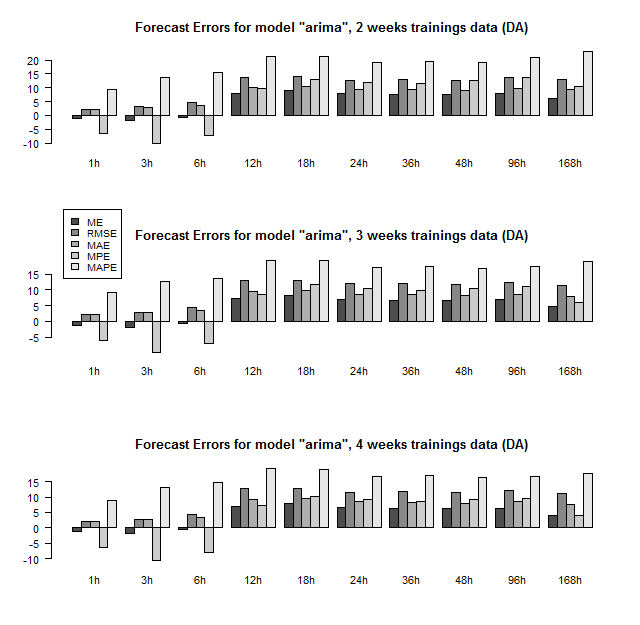
\includegraphics[width=0.85\textwidth]{figures/forecasting/da_sim_1_x_1w_1w_arima.png}
	\caption{Aggregated accuracy measures for ARIMA model and training data of 2, 3 and 4 weeks, Nord Pool Spot, Hamina}
	\label{fig:da_sim_1_x_1w_1w_arima}
\end{figure}

\begin{figure}[htbp]
	\centering
		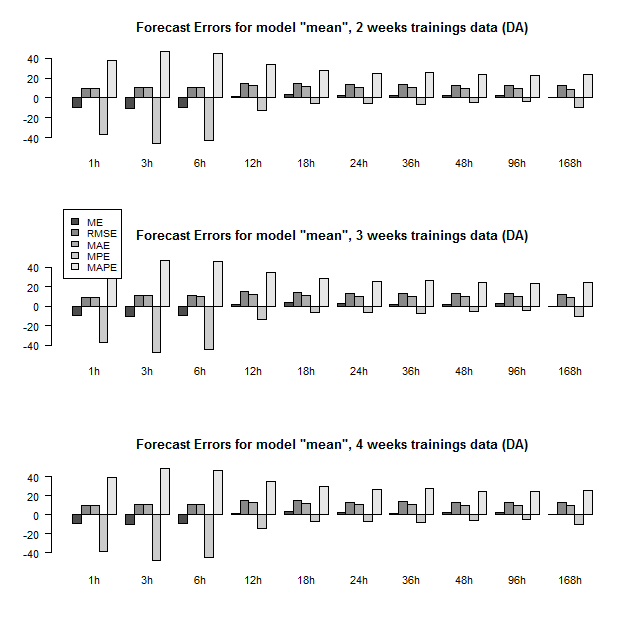
\includegraphics[width=0.85\textwidth]{figures/forecasting/da_sim_1_x_1w_1w_mean.png}
	\caption{Aggregated accuracy measures for Mean model and training data of 2, 3 and 4 weeks, Nord Pool Spot, Hamina}
	\label{fig:da_sim_1_x_1w_1w_mean}
\end{figure}


The result tables as well as graphs emphasize the observations made previously about model behavior. 

What can be observed by investigating the large scale forecast evaluation over all locations is that very different behaviors and scales of forecast errors exist for the same model over different locations (i.e.~datasets). An extreme example is the difference in forecast error distributions of the Nord Pool Spot and Belpex energy markets (tables \ref{ssec:app_tables_nord_pool_spot} and \ref{ssec:app_tables_belpex}, graphs \ref{ssec:app_graphs_nord_pool_spot} and \ref{ssec:app_graphs_belpex}). 

However, the seemingly extreme difference in forecast error distribution is mainly caused by exorbitant values of the MPE and MAPE error measures. This may be attributed to the occurrence of many low valued energy prices (close to zero) in the Belpex energy market which causes very high values for these methods. 

When comparing models TBATS, ARIMA followed by Mean and SES forecast models achieve the best results. Remarkably Mean forecasts outperform forecasts of SES models for almost all data sets of day ahead energy markets regarding forecast horizons $>= 12$. This behavior is reversed for real time markets where SES generally provides better performance. 

TBATS models exhibit the least forecast errors when they are able to capture seasonality appropriately. Otherwise these models show exponential growth of forecast errors over all measures. Due to this instability ARIMA models may be preferred as they exhibit stable forecast errors over most data sets and forecast horizons. 

Another note to error distribtions is that for the same forecast model similar patterns can be observed despite differences across energy markets. Concerning different training periods it can be observed that for most methods errors decrease with increasing training period, i.e.~four weeks of training data exhibits the least errors in most cases. 

Also different distributions are apparent for different error measures, e.g.~RMSE tend to increase with increasing forecast horizon whereas percentage errors (MPE and MAPE) tend to hit their lowest values for forecast horizons of 24h to 48h apart from horizons below 12h. 

Concerning the forecast error measures a focus has been laid on evaluating Root Mean Squared Errors (RMSE) since this measure has been proven to provide the most stable results. Percentage error measures such as Mean Percentage Error (MPE) and Mean Absolute Percentage Error (MAPE) tend to become numerically unstable for low values. Difference based measures such as Mean Error (ME) with non-absolute value differences provide little insights to the actual occurred forecast errors as positive and negative values might cancel each other out. 



\subsubsection{Aggregated Results}

Results have been aggregated over all forecast horizons and for each simulation which are shown in Tables \ref{tab:aggregated_results_nord_pool}, \ref{tab:aggregated_results_belpex}, \ref{tab:aggregated_results_isone} and \ref{tab:aggregated_results_pjm}. Best results have been formatted in bold in the tables. 

ARIMA and TBATS models showed superior results over all forecast horizons and training periods. TBATS models show best results when data can be modeled appropriately but exhibit anomalies in other cases. For different training periods a trend can be detected where forecast errors increase with increasing duration of the training period. However, ARIMA models show opposite results where forecast errors consistently decrease with increasing training period. 


% latex table generated in R 3.1.1 by xtable 1.8-2 package
% Fri Mar 25 19:35:50 2016
\begin{table}[ht]
\centering
\begin{tabular}{rrrrrrr}
  \hline
 & mean & ses & holts & holtwinters & arima & tbats \\ 
  \hline
2 weeks & 12.37 & 11.60 & 62.76 & 73.98 & 10.22 & \textbf{8.21} \\ 
  3 weeks & 12.57 & 11.60 & 62.90 & 75.55 & 9.50 & \textbf{8.57} \\ 
  4 weeks & 12.72 & 11.60 & 63.23 & 85.85 & 9.26 & \textbf{8.43} \\ 
   \hline
\end{tabular}
\caption{Results of evaluation for Hamina, Nord Pool Spot (DA)} 
\label{tab:aggregated_results_nord_pool}
\end{table}
% latex table generated in R 3.1.1 by xtable 1.8-2 package
% Fri Mar 25 19:35:50 2016
\begin{table}[ht]
\centering
\begin{tabular}{rrrrrrr}
  \hline
 & mean & ses & holts & holtwinters & arima & tbats \\ 
  \hline
2 weeks & 15.77 & 15.23 & 127.13 & 186.82 & \textbf{13.49} & 1.27E+50 \\ 
  3 weeks & 16.07 & 15.27 & 128.05 & 190.86 & 12.94 & \textbf{11.61} \\ 
  4 weeks & 16.25 & 15.30 & 127.03 & 186.37 & \textbf{12.87} & 2.49E+36 \\ 
   \hline
\end{tabular}
\caption{Results of evaluation for St.Ghislain, Belpex (DA)}
\label{tab:aggregated_results_belpex}
\end{table}
% latex table generated in R 3.1.1 by xtable 1.8-2 package
% Fri Mar 25 19:35:50 2016
\begin{table}[ht]
\centering
\begin{tabular}{rrrrrrr}
  \hline
 & mean & ses & holts & holtwinters & arima & tbats \\ 
  \hline
2 weeks & 26.42 & 23.61 & 235.84 & 417.39 & \textbf{24.11} & 5.45E+16 \\ 
  3 weeks & 26.36 & 23.56 & 238.92 & 686.95 & \textbf{22.26} & 1.64E+18 \\ 
  4 weeks & 26.84 & 23.32 & 268.10 & 437.85 & \textbf{21.83} & 2.18E+32 \\ 
   \hline
\end{tabular}
\caption{Results of evaluation for Portland, ISO-NE (RT)}
\label{tab:aggregated_results_isone}
\end{table}
% latex table generated in R 3.1.1 by xtable 1.8-2 package
% Fri Mar 25 19:35:50 2016
\begin{table}[ht]
\centering
\begin{tabular}{rrrrrrr}
  \hline
 & mean & ses & holts & holtwinters & arima & tbats \\ 
  \hline
2 weeks & 17.41 & 15.17 & 148.54 & 333.32 & \textbf{15.02} & 7.57E+13 \\ 
  3 weeks & 17.36 & 15.23 & 147.77 & 318.61 & 14.14 & \textbf{ 13.46} \\ 
  4 weeks & 17.34 & 15.29 & 148.67 & 357.82 & \textbf{14.11} & 5.44E+108 \\  
   \hline
\end{tabular}
\caption{Results of evaluation for Richmond, PJM (RT)}
\label{tab:aggregated_results_pjm}
\end{table}



\subsection{Conclusion of results}

From the discussion of the large scale forecast evaluation in the previous section various conclusions may be drawn. 

\paragraph{Model performance}

Concerning model performance ARIMA models showed the best results over different energy markets, training periods and forecast horizons. 
They showed consistently low forecast errors and appeared very stable throughout the simulations. Thus among the observed models ARIMA models may be the best choice considering forecast performance and statbility of results. 

\paragraph{Forecast Horizon}

Concerning forecast horizons it has been observed that horizons from 24 hours to 48 hours provide the best results when considering all models and training periods. 
For low horizons up to 12 hours different models may be suggested, i.e.~Holts model provide considerably lower forecast errors for forecast windows of 1 and 3 hours. 
For other than very short-term forecasts a forecast window of 24 to 48 hours provides best results. 

\paragraph{Training periods}

Different model training periods provide different results. Forecast errors have been observed to increase with the duration of the training period most of the time except for ARIMA models where the opposite behavior has been detected. Thus for ARIMA models a training period of 4 weeks is suggested for model generation. 

\paragraph{Forecast error measures}

As discussed before different forecast error methods provide different results for the same dataset. The ME provides an indication of the symmetry of the error distribution but little information about actual forecast performance. The MAE and RMSE provide a way of reliably model forecast errors where they achieve very similar results while the RMSE emphasizes outliers in the data. Percentage error measures have not been found to provide a reliable source of error measurements due to their instability for low values. Thus MAE and RMSE are considered the preferred way of modeling forecast errors. 






